\def\pgfsysdriver{pgfsys-dvisvgm.def}
\documentclass[tikz,border=4pt]{standalone}
\usepackage{amsmath}
\usetikzlibrary{calc}
% Semantic palette shared by the light and dark exports; geometry and TeX glyphs stay identical.
\ifdefined\FigureDark
  \definecolor{FigureForeground}{HTML}{E1E8DF}
  \definecolor{FigureMuted}{HTML}{94A69B}
  \definecolor{FigureBlue}{HTML}{8CC5F2}
  \definecolor{FigureOrange}{HTML}{F4B76B}
  \definecolor{FigureRed}{HTML}{F28E86}
  \definecolor{FigureBlueFill}{HTML}{273F4F}
  \definecolor{FigureOrangeFill}{HTML}{4A3726}
  \definecolor{FigurePaper}{HTML}{1B2420}
\else
  \definecolor{FigureForeground}{HTML}{202C29}
  \definecolor{FigureMuted}{HTML}{68766E}
  \definecolor{FigureBlue}{HTML}{245A88}
  \definecolor{FigureOrange}{HTML}{986000}
  \definecolor{FigureRed}{HTML}{A44030}
  \definecolor{FigureBlueFill}{HTML}{E5EDF8}
  \definecolor{FigureOrangeFill}{HTML}{FFF0D8}
  \definecolor{FigurePaper}{HTML}{FBFAF7}
\fi

\begin{document}
% Coordinate sketches, NOT isometric Euclidean developments of the meshes.
% Identical S, p and oriented boundary in all panels. Orange circles are
% schematic atomic curvature contributions; orange shading is a density.
% At refinement, interior marker area is approximately held constant (9 versus 37 sites).
% No deficit is computed from the visibly planar triangle angles.
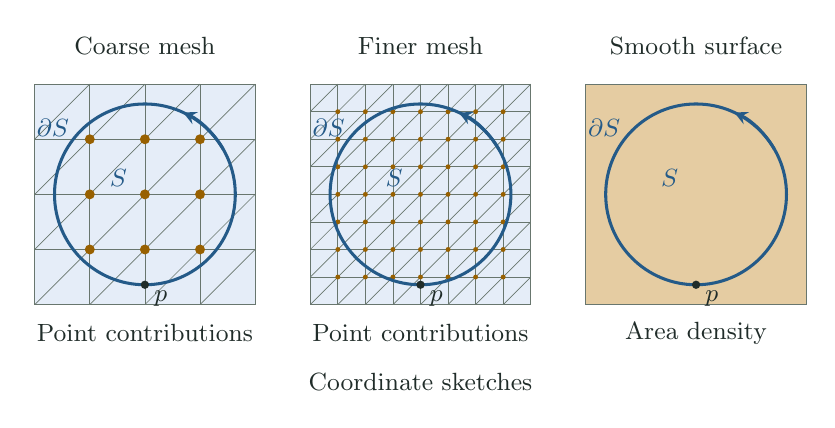
\begin{tikzpicture}[x=1.4cm,y=1.4cm,color=FigureForeground,font=\small,>=stealth]
\foreach \panel/\shift/\heading in {0/0/Coarse mesh,1/3.5/Finer mesh,2/7/Smooth surface}{
 \begin{scope}[xshift=\shift cm]
 \node at (0,1.35) {\textnormal{\heading}};
 \ifnum\panel<2
  \fill[FigureBlueFill] (-1,-1) rectangle(1,1);
  \ifnum\panel=0 \def\step{.5}\def\radius{1.8pt}
  \else \def\step{.25}\def\radius{.888pt}\fi
  % Triangles belong to the coordinate image of the mesh, not its metric.
  \foreach \i in {0,...,8}{
   \pgfmathsetmacro{\z}{-1+\i*\step}
   \ifdim\z pt<1.001pt
    \draw[FigureMuted,line width=.25pt] (\z,-1)--(\z,1) (-1,\z)--(1,\z);
   \fi
  }
  \foreach \i in {0,...,7}{\foreach \j in {0,...,7}{
   \pgfmathsetmacro{\xx}{-1+\i*\step}
   \pgfmathsetmacro{\yy}{-1+\j*\step}
   \pgfmathsetmacro{\endx}{\xx+\step}
   \pgfmathsetmacro{\endy}{\yy+\step}
   \ifdim\endx pt<1.001pt\ifdim\endy pt<1.001pt
    \draw[FigureMuted,line width=.25pt] (\xx,\yy)--(\endx,\endy);
   \fi\fi
  }}
  % Only internal chart vertices carry markers. Membership in S is set by
  % the common circle. Excluded fine-grid atoms remain visibly outside it.
  \foreach \i in {1,...,7}{\foreach \j in {1,...,7}{
   \pgfmathsetmacro{\xx}{-1+\i*\step}
   \pgfmathsetmacro{\yy}{-1+\j*\step}
   \ifdim\xx pt<.999pt\ifdim\yy pt<.999pt
    \fill[FigureOrange] (\xx,\yy) circle(\radius);
   \fi\fi
  }}
 \else
  % A continuous scalar density on the chart, with no vertex atoms.
  \fill[FigureOrangeFill!75!FigureOrange]
   (-1,-1) rectangle(1,1);
 \fi
 \draw[FigureMuted,line width=.35pt] (-1,-1) rectangle(1,1);
 % The same coordinate boundary and basepoint in all three views.
 \draw[FigureBlue,line width=1.1pt] (0,0) circle(.82);
 \draw[FigureBlue,line width=1.1pt,->] (30:.82) arc(30:65:.82);
 \fill[FigureForeground] (0,-.82) circle(1.5pt);
 \node[FigureBlue,anchor=north east] at (-.6,.77) {$\partial S$};
 \node[FigureBlue] at (-.24,.15) {$S$};
 \node[anchor=north west,inner sep=2pt] at (.03,-.82) {$p$};
 \ifnum\panel<2
  \node at (0,-1.26) {\textnormal{Point contributions}};
 \else
  \node at (0,-1.26) {\textnormal{Area density}};
 \fi
 \end{scope}
}
\node at (3.5cm,-1.70) {\textnormal{Coordinate sketches}};
\end{tikzpicture}
\end{document}
